\documentclass{article}
% \documentclass{beamer}
% \usetheme{Madrid}

%------------------------------
% used for href/url
\usepackage{hyperref}


% used for math fomulas
\usepackage{amsmath}

% used for pictures
\usepackage{graphicx}
\usepackage{subcaption}
\usepackage{float}

% used for codes
\usepackage{listings}
\lstset{
  basicstyle=\ttfamily\footnotesize, % Set your code to be drawn with a monospaced font
  breaklines=true, % Enables line breaking
  frame=single % Adds a frame around the code
}

% used for Graph
\usepackage{adigraph}

% used for Bayesian Network
\usepackage{tikz}
\usetikzlibrary{bayesnet}

%------------------------------
% TODO 
\tolerance=10000
\emergencystretch=\maxdimen
\hyphenpenalty=10000
\hbadness=10000


\usepackage{silence}
\WarningFilter{latex}{Overfull \hbox}

%------------------------------



\title{MK's Notes for CIVL-4530 Geometric Design}
\date{2024-03-04}
\author{Michael Chen}

\begin{document}
  \pagenumbering{gobble}
  \maketitle
  \newpage
  \pagenumbering{roman}


  % ----------------------------------------
  \tableofcontents
  \newpage


  % ----------------------------------------
  Geometric Design is a basic course of Transportation, introducing principal concepts and fomulas.

  \newpage

  % ----------------------------------------
  \setcounter{section}{0}
  \section{Chapter 01 Introduction and Highway Function}
  \subsection{Objectives}
  \begin{enumerate}
    \item Geometric Design concepts
    \item Highway Funciton
  \end{enumerate}

  \subsection{Geometric Design Definition}
  \begin{enumerate}
    \item fit the highway to the terrain
    \item maintaining design standards for safety and performance
  \end{enumerate}

  \subsection{Geometric Design Basic}
  \begin{enumerate}
    \item make criteria matches  
    \begin{enumerate}
      \item driver expectancy/behavior
      \item vehicle performance/behavior
    \end{enumerate}
    \item balance safty, cost, mobility, community values, environmental, politics, liability, sustainable development, etc
  \end{enumerate}

  \subsection{AASHTO Role}
  \begin{enumerate}
    \item American Association of State Highway and Transportation Officials
    \item the membership of AASHTO consists of FHWA, and state DOTs
  \end{enumerate}

  % ----------------------------------------
  \subsection{Reference - AASHTO publications}
  \begin{enumerate}
    \item \textbf{a.k.a Green Book/PGDHS:} A Policy on Geometric Design of Highways and Streets, 2018, 7th Edition
    \item Guidelines for Geometric Design of Very Low Volume Local Roads, 2001
    \item A Guide to Achieving Flexibility in Highway Design, May 2004
    \item Guide for the Planning, Design, and Operation of Pedestrian Facilities, July 2004
    \item Guide for the Development of Bicycle Facilities, June 2012

    \item Good for New Highway Design 
    \item TRB Special Report 214, Designing Safer Roads: Practices for Resurfacing, Restoration, and Rehabilitation for guidance. \\
  \end{enumerate}

  \subsection{Reference - ITE publications}
  \begin{enumerate}
    \item Urban Street Geometric Design Handbook, 2008
    \item Freeway and Interchange Geometric Design Handbook, 2007
    \item Designing Walkable Urban Thoroughfares: A Context Sensitive Approach, March 2010
  \end{enumerate}

  % ------------------ todo

  \subsection{Older Driver Deficiencies}


  \begin{tabular}{|c|c|c|c|c|}
    Roadway & urban & rural level & rural rolling & rural mountainous\\
    \hline
    Freeway & C/D   & B & B & C\\
    Arterial & C/D  & B & B & C\\
    Collector & D   & C & C & D\\
    Local & D       & D & D & D\\
  \end{tabular}
  \begin{figure}[h!]
    \includegraphics[width=\linewidth]{LOS.png}
    \caption{Level of Service}
    \label{fig:image-LOS}
  \end{figure}

  \subsection{13 AASHTO Criteria}
  \begin{enumerate}
      \item design speed
      \item lane width
      \item shoulder width
      \item bridge width
      \item structural capacity
      \item 
      \item horizontal alignment
      \item vertical alignment
      \item cross slope
      \item grades
      \item superelevation
      \item horizontal clearance
      \item vertical clearance
  \end{enumerate}

  \subsection{speed}
  \begin{enumerate}
    \item running speed - the speed of an individual vehicle
    \item design speed - AASHTO: max safe speed
    \item operation speed - the 85th percentile of observed speed in free flow conditions
    \item safty of over speed - $\Delta$V: [0, 5] low; [5, 15] medium; [15, infinit] high
  \end{enumerate}

  minimum design speed for \textbf{rural} roadways vs vehicle per day(VPD)
  \begin{tabular}{|c|c|c|c|}
    \hline
    rural terrain & 0-400 & 400-2000 & over 2000 \\
    \hline
    level         & 40    & 50       & 60 \\
    rolling       & 30    & 40       & 50 \\
    mountainous   & 20    & 30       & 40 \\
  \end{tabular}

  \subsection{lane width for urban and rural (1-2ft wider than urban)}
  \begin{tabular}{|l|l|l|}
    Types & urban & rural \\
    \hline
    Freeway and Interstates: & 12ft, & 12ft\\
    Ramp: & 12-30ft & 12-30ft \\ 
    Arterial: & 11-12ft, & 10-12ft \\
    Collections: & 10-12ft, & 10-12ft\\
    local roads: & 9-12ft, & 9-12ft  \\
  \end{tabular}

  \subsection{cross slope}
  paved surfaces: 1.5-2\%, typical 2\%  - Green Book\\
  unpaved surfaces: 2-6\% - Green Book\\
  areas with high intensity rainfall: 2-2.5\% \\
  ALDOT use in 2 Counties: 2.2\% \\



\begin{table}[ht]
\centering
\caption{Lane Widths for Different Types of Roadways}
\label{tab:lane_widths}
\begin{tabular}{@{}lcccc@{}}
\hline
\textbf{Type of Roadway} & \multicolumn{2}{c}{\textbf{Rural}} & \multicolumn{2}{c}{\textbf{Urban}} \\
                         & \textbf{US (feet)} & \textbf{Metric (meters)} & \textbf{US (feet)} & \textbf{Metric (meters)} \\ 
\hline
Freeway                  & 14-16*             & 4.3-4.9*                & 14–16*             & 4.3–4.9*                \\
Arterial                 & 14-16              & 4.3-4.9                 & 14–16              & 4.3–4.9                 \\
Collector                & 14                 & 4.3                     & 14                 & 4.3                     \\
Local                    & 14                 & 4.3                     & 14                 & 4.3                     \\
\hline
\end{tabular}
\end{table}




\begin{table}[ht]
\centering
\caption{Functional Classification of Roadways}
\label{tab:functional_classification}
\begin{tabular}{@{}lccc@{}}
\hline
\textbf{Criteria} & \textbf{Local} & \textbf{Collector} & \textbf{Arterial} \\
\hline
Street pavement width & 24 ft & 22 ft (1), 31 ft & 36 ft (2), 48 ft \\
Minimum horizontal curve radius & 200 ft & 350 ft & 550 ft \\
Maximum grade (3) & 15\% & 12\% & 8\% \\
Minimum design speed for vertical curve & 25 mi/h & 35 mi/h & 45 mi/h \\
\hline
\end{tabular}
\end{table}


  % ----------------------------------------
  \subsection{Terms}
  SU - represents all single unit trucks and small buses, with length 35-60ft \\
  ADT - average daily traffic \\
  AADT - the annual average daily traffic, empersizing annual average \\
  DHV - design hour volume \\
  DDHV - The directional design hour volume \\
  30HV - the 30th Highest Hour of Yearly Traffic - the 30th Hour volume \\
  design speed (DS) - design maximum speed of a roadway \\
  free flow speed (FFS) - the observed speed at which vehicles can travel with minimal delays and no restrictions from traffic signals, congestion, or other factors. \\
  LOS - Characterization of operating conditions, related to speed, travel time, traffic density, freedom to maneuver  \\
  FFS is close to DS - It means a good design \\
  K-factor - DHV = K * ADT, K is 8 to 12\% for urban facilities; 12 to 18\% for rural facilities.  \\
  D-factor - DDHV = D * DHV, D is 50\% for urban highways; 55 - 80\% for rural and suburban roads \\
  DDHV = ADT (or AADT) * K * D \\
  CMF - Crash Modification Factor \\
  Cul-de-sac: deed end street \\

  \subsection{Rules}
  Tandem Axle - 2 axles which are very close\\
  State maximum gross vehicle weight - 73,280 - 164,000 lbs\\
  State maximum gross vehicle weight - 73,280 - 164,000 lbs\\
  \\
  DHV = 8\% - 12\% ADT in urban area, refer to Green Book\\
  30HV = 15\% ADT in a typical rural arterial, refer to Green Book\\

  % ----------------------------------------
  \subsection{Formulas}
  1 mile = 5,280 feet \\
  1000 kg = 2204.62 lbs \\
  1 foot = 0.3048 meters \\
  1 lb = 16 oz \\
  1 gallon = 3.785 liters (U.S. liquid gallon) \\
  1 gallon = 4.546 liters (U.K. imperial gallon) \\


  % ----------------------------------------
  \subsection{Reference}
  FHWA Website \\
  http://safety.fhwa.dot.gov/geometric/pubs/mitigationstrategies/ \\

  \newpage

  % ----------------------------------------
  \section{Writing Formulas}
  \subsection{Equation - ONLY support one formula per line}
  \begin{equation}
    formula 1: f(x) = x^2   ----
    formula 2: \prod_{2}^{n}
  \end{equation}

  \subsection{Align - support MULTIPLE formulas in the same block}
  NOTE: need use package amsmath to enable Align 
  \begin{align*}
    f(x) &= x & 2 \\
    g(x) &= \frac{1}{x} \\
    F(x) = f(x) + g(x) &= \int_{a}^{b} \frac{1}{3}x^3 \\
    W(x) &= \frac{1}{\sqrt{x}} + \frac{1}{\sqrt[3]{y}} \\
    Z(x) &= \left( 3 + 2 \right) * 2
  \end{align*}
  \subsubsection{}
  So which one, align or equation, will you use?


  \subsection{Inline math}
  The form is used for $ f(x) = x^ 2 $ or $\lambda$, so you can easily to use them. 
  https://github.com/LucaCappelletti94/adigraph
  \subsection{Matrics}
  $
  \left[
  \begin{matrix}
    3 & 2 \\
    9 & 4 & x
  \end{matrix}
  \right]
  $

  \newpage


  % ----------------------------------------
  \section{Embedding Pictures/Figures}

  \subsection{One figure}
  NOTE: need to use package graphicshttps://github.com/LucaCappelletti94/adigraph to enable figure

  \begin{figure}[h!]
    % \includegraphics[width=\linewidth]{}
    \caption{Auburn Campus}
    \label{fig:au01}
  \end{figure}

  \subsection{Multiple figures}
  NOTE: need to use package subcaption to enable Multiple figures.
  Here are figures:
  \begin{figure}[H]
    \centering
    \begin{subfigure}[b]{0.4\linewidth}
      % \includegraphics[width=\linewidth]{}
      \caption{Auburn Overview}
    \end{subfigure}
    \begin{subfigure}[b]{0.4\linewidth}
      % \includegraphics[width=\linewidth]{}
      \caption{Auburn Buildings}
    \end{subfigure}
    \caption{Two Auburn Old Pictures}
    \label{fig:twoPic}
  \end{figure}

  \subsection{Use float and H}
  Use package float and attribute H to strictly fix the pictures' posisiton to HERE.

  \begin{lstlisting}[caption={An Example}]
    \usepackage{float}
    ...


    \begin{figure}[H]
      ....
    \end{figure}

    
  \end{lstlisting}
  \newpage


  % ----------------------------------------

  \section{Drawing Bayesian Network and Graph}
  \subsection{Use pagckages: tikz and bayesnet}
  Use 2 packages: tikz and bayesnet to draw Bayesian Network chat.
  \break

  Type 1:
  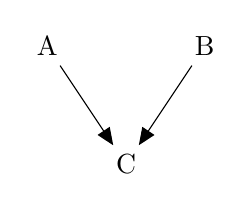
\begin{tikzpicture}
  \node (A) at (0,0) {A};
  \node (B) at (2,0) {B};
  \node (C) at (1,-1.5) {C};
  \draw[->] (A) -- (C);
  \draw[->] (B) -- (C);
  \end{tikzpicture}


  Type 2:
  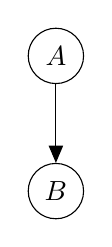
\begin{tikzpicture}
  \node[latent] (A) {$A$};
  \node[latent, below = of A] (B) {$B$};
  \edge {A} {B};
  \end{tikzpicture}
  \iffalse
  \fi
  
 
  \subsection{Use pagckages: adigraph}

  \NewAdigraph{myAdigraph}{
    s:0,0;
    1:2,2;
    3:2,-2;
    2:6,2;
    4:6,-2;
    t:8,0;
}{
    s,1:25;
    s,3:25;
    3,4:25;
    1,2:35;
    2,t:20;
    4,t:30;
    3,1:10;
    4,2:10;
    2,3:15::near start;
    4,1:5::near start;
}
\myAdigraph{}

\newpage


% --------------------------------------
\section{Using packages}
Packages are like plugins to extend the Latex' capabilities. Some common commands are listed here.

\begin{lstlisting}[language=bash, caption={tlmgr commands and etc}]
tlmgr list --only-installed   # show installed packages

tlmgr search <package-name>   # search a packages
tlmgr info <package-name>     # show a package's intro, no matter installed or not
tlmgr install <package-name>  # install a new packages

tlmgr update --self --all     # update package index

kpsewhich article.sty         # locate a package's .sty file

# env variables can define additional directories to be searched. 
echo $TEXMFHOME $TEXMFLOCAL $TEXMFSYSCONFIG 
\end{lstlisting}
\newpage


% --------------------------------------
\section{Generate Slides}
Use the package beamer to generate a pdf file of slides from an article


\begin{lstlisting}[caption={Changes in .tex file}]
  % \documentclass{article}
  \documentclass{beamer}
  \usetheme{Madrid}
\end{lstlisting}

% --------------------------------------
\end{document}